\documentclass[twoside]{book}

% Packages required by doxygen
\usepackage{fixltx2e}
\usepackage{calc}
\usepackage{doxygen}
\usepackage[export]{adjustbox} % also loads graphicx
\usepackage{graphicx}
\usepackage[utf8]{inputenc}
\usepackage{makeidx}
\usepackage{multicol}
\usepackage{multirow}
\PassOptionsToPackage{warn}{textcomp}
\usepackage{textcomp}
\usepackage[nointegrals]{wasysym}
\usepackage[table]{xcolor}

% Font selection
\usepackage[T1]{fontenc}
\usepackage[scaled=.90]{helvet}
\usepackage{courier}
\usepackage{amssymb}
\usepackage{sectsty}
\renewcommand{\familydefault}{\sfdefault}
\allsectionsfont{%
  \fontseries{bc}\selectfont%
  \color{darkgray}%
}
\renewcommand{\DoxyLabelFont}{%
  \fontseries{bc}\selectfont%
  \color{darkgray}%
}
\newcommand{\+}{\discretionary{\mbox{\scriptsize$\hookleftarrow$}}{}{}}

% Page & text layout
\usepackage{geometry}
\geometry{%
  a4paper,%
  top=2.5cm,%
  bottom=2.5cm,%
  left=2.5cm,%
  right=2.5cm%
}
\tolerance=750
\hfuzz=15pt
\hbadness=750
\setlength{\emergencystretch}{15pt}
\setlength{\parindent}{0cm}
\setlength{\parskip}{3ex plus 2ex minus 2ex}
\makeatletter
\renewcommand{\paragraph}{%
  \@startsection{paragraph}{4}{0ex}{-1.0ex}{1.0ex}{%
    \normalfont\normalsize\bfseries\SS@parafont%
  }%
}
\renewcommand{\subparagraph}{%
  \@startsection{subparagraph}{5}{0ex}{-1.0ex}{1.0ex}{%
    \normalfont\normalsize\bfseries\SS@subparafont%
  }%
}
\makeatother

% Headers & footers
\usepackage{fancyhdr}
\pagestyle{fancyplain}
\fancyhead[LE]{\fancyplain{}{\bfseries\thepage}}
\fancyhead[CE]{\fancyplain{}{}}
\fancyhead[RE]{\fancyplain{}{\bfseries\leftmark}}
\fancyhead[LO]{\fancyplain{}{\bfseries\rightmark}}
\fancyhead[CO]{\fancyplain{}{}}
\fancyhead[RO]{\fancyplain{}{\bfseries\thepage}}
\fancyfoot[LE]{\fancyplain{}{}}
\fancyfoot[CE]{\fancyplain{}{}}
\fancyfoot[RE]{\fancyplain{}{\bfseries\scriptsize Generated by Doxygen }}
\fancyfoot[LO]{\fancyplain{}{\bfseries\scriptsize Generated by Doxygen }}
\fancyfoot[CO]{\fancyplain{}{}}
\fancyfoot[RO]{\fancyplain{}{}}
\renewcommand{\footrulewidth}{0.4pt}
\renewcommand{\chaptermark}[1]{%
  \markboth{#1}{}%
}
\renewcommand{\sectionmark}[1]{%
  \markright{\thesection\ #1}%
}

% Indices & bibliography
\usepackage{natbib}
\usepackage[titles]{tocloft}
\setcounter{tocdepth}{3}
\setcounter{secnumdepth}{5}
\makeindex

% Hyperlinks (required, but should be loaded last)
\usepackage{ifpdf}
\ifpdf
  \usepackage[pdftex,pagebackref=true]{hyperref}
\else
  \usepackage[ps2pdf,pagebackref=true]{hyperref}
\fi
\hypersetup{%
  colorlinks=true,%
  linkcolor=blue,%
  citecolor=blue,%
  unicode%
}

% Custom commands
\newcommand{\clearemptydoublepage}{%
  \newpage{\pagestyle{empty}\cleardoublepage}%
}

\usepackage{caption}
\captionsetup{labelsep=space,justification=centering,font={bf},singlelinecheck=off,skip=4pt,position=top}

%===== C O N T E N T S =====

\begin{document}

% Titlepage & ToC
\hypersetup{pageanchor=false,
             bookmarksnumbered=true,
             pdfencoding=unicode
            }
\pagenumbering{roman}
\begin{titlepage}
\vspace*{7cm}
\begin{center}%
{\Large Slang \\[1ex]\large 0.\+1 }\\
\vspace*{1cm}
{\large Generated by Doxygen 1.8.11}\\
\end{center}
\end{titlepage}
\clearemptydoublepage
\tableofcontents
\clearemptydoublepage
\pagenumbering{arabic}
\hypersetup{pageanchor=true}

%--- Begin generated contents ---
\chapter{Hierarchical Index}
\section{Class Hierarchy}
This inheritance list is sorted roughly, but not completely, alphabetically\+:\begin{DoxyCompactList}
\item \contentsline{section}{slang\+\_\+\+A\+S\+T\+\_\+\+N\+O\+D\+ES\+:\+:Expression}{\pageref{classslang__AST__NODES_1_1Expression}}{}
\begin{DoxyCompactList}
\item \contentsline{section}{slang\+\_\+\+A\+S\+T\+\_\+\+N\+O\+D\+ES\+:\+:Binary\+Operation}{\pageref{classslang__AST__NODES_1_1BinaryOperation}}{}
\item \contentsline{section}{slang\+\_\+\+A\+S\+T\+\_\+\+N\+O\+D\+ES\+:\+:Function\+Call}{\pageref{classslang__AST__NODES_1_1FunctionCall}}{}
\item \contentsline{section}{slang\+\_\+\+A\+S\+T\+\_\+\+N\+O\+D\+ES\+:\+:Identifier}{\pageref{classslang__AST__NODES_1_1Identifier}}{}
\item \contentsline{section}{slang\+\_\+\+A\+S\+T\+\_\+\+N\+O\+D\+ES\+:\+:Literal}{\pageref{classslang__AST__NODES_1_1Literal}}{}
\end{DoxyCompactList}
\item \contentsline{section}{slang\+\_\+\+A\+S\+T\+\_\+\+N\+O\+D\+ES\+:\+:Function}{\pageref{classslang__AST__NODES_1_1Function}}{}
\item \contentsline{section}{slang\+\_\+\+A\+S\+T\+\_\+\+N\+O\+D\+ES\+:\+:Operator}{\pageref{classslang__AST__NODES_1_1Operator}}{}
\begin{DoxyCompactList}
\item \contentsline{section}{slang\+\_\+\+A\+S\+T\+\_\+\+N\+O\+D\+ES\+:\+:For\+Loop}{\pageref{classslang__AST__NODES_1_1ForLoop}}{}
\item \contentsline{section}{slang\+\_\+\+A\+S\+T\+\_\+\+N\+O\+D\+ES\+:\+:Operators}{\pageref{classslang__AST__NODES_1_1Operators}}{}
\item \contentsline{section}{slang\+\_\+\+A\+S\+T\+\_\+\+N\+O\+D\+ES\+:\+:Op\+Expression}{\pageref{classslang__AST__NODES_1_1OpExpression}}{}
\item \contentsline{section}{slang\+\_\+\+A\+S\+T\+\_\+\+N\+O\+D\+ES\+:\+:Op\+IF}{\pageref{classslang__AST__NODES_1_1OpIF}}{}
\item \contentsline{section}{slang\+\_\+\+A\+S\+T\+\_\+\+N\+O\+D\+ES\+:\+:Op\+Return}{\pageref{classslang__AST__NODES_1_1OpReturn}}{}
\item \contentsline{section}{slang\+\_\+\+A\+S\+T\+\_\+\+N\+O\+D\+ES\+:\+:While\+Loop}{\pageref{classslang__AST__NODES_1_1WhileLoop}}{}
\end{DoxyCompactList}
\end{DoxyCompactList}

\chapter{Class Index}
\section{Class List}
Here are the classes, structs, unions and interfaces with brief descriptions\+:\begin{DoxyCompactList}
\item\contentsline{section}{\hyperlink{classslang__AST__NODES_1_1BinaryOperation}{slang\+\_\+\+A\+S\+T\+\_\+\+N\+O\+D\+E\+S\+::\+Binary\+Operation} }{\pageref{classslang__AST__NODES_1_1BinaryOperation}}{}
\item\contentsline{section}{\hyperlink{classslang__AST__NODES_1_1Expression}{slang\+\_\+\+A\+S\+T\+\_\+\+N\+O\+D\+E\+S\+::\+Expression} }{\pageref{classslang__AST__NODES_1_1Expression}}{}
\item\contentsline{section}{\hyperlink{classslang__AST__NODES_1_1ForLoop}{slang\+\_\+\+A\+S\+T\+\_\+\+N\+O\+D\+E\+S\+::\+For\+Loop} }{\pageref{classslang__AST__NODES_1_1ForLoop}}{}
\item\contentsline{section}{\hyperlink{classslang__AST__NODES_1_1Function}{slang\+\_\+\+A\+S\+T\+\_\+\+N\+O\+D\+E\+S\+::\+Function} }{\pageref{classslang__AST__NODES_1_1Function}}{}
\item\contentsline{section}{\hyperlink{classslang__AST__NODES_1_1FunctionCall}{slang\+\_\+\+A\+S\+T\+\_\+\+N\+O\+D\+E\+S\+::\+Function\+Call} }{\pageref{classslang__AST__NODES_1_1FunctionCall}}{}
\item\contentsline{section}{\hyperlink{classslang__AST__NODES_1_1Identifier}{slang\+\_\+\+A\+S\+T\+\_\+\+N\+O\+D\+E\+S\+::\+Identifier} }{\pageref{classslang__AST__NODES_1_1Identifier}}{}
\item\contentsline{section}{\hyperlink{classslang__AST__NODES_1_1Literal}{slang\+\_\+\+A\+S\+T\+\_\+\+N\+O\+D\+E\+S\+::\+Literal} }{\pageref{classslang__AST__NODES_1_1Literal}}{}
\item\contentsline{section}{\hyperlink{classslang__AST__NODES_1_1Operator}{slang\+\_\+\+A\+S\+T\+\_\+\+N\+O\+D\+E\+S\+::\+Operator} }{\pageref{classslang__AST__NODES_1_1Operator}}{}
\item\contentsline{section}{\hyperlink{classslang__AST__NODES_1_1Operators}{slang\+\_\+\+A\+S\+T\+\_\+\+N\+O\+D\+E\+S\+::\+Operators} }{\pageref{classslang__AST__NODES_1_1Operators}}{}
\item\contentsline{section}{\hyperlink{classslang__AST__NODES_1_1OpExpression}{slang\+\_\+\+A\+S\+T\+\_\+\+N\+O\+D\+E\+S\+::\+Op\+Expression} }{\pageref{classslang__AST__NODES_1_1OpExpression}}{}
\item\contentsline{section}{\hyperlink{classslang__AST__NODES_1_1OpIF}{slang\+\_\+\+A\+S\+T\+\_\+\+N\+O\+D\+E\+S\+::\+Op\+IF} }{\pageref{classslang__AST__NODES_1_1OpIF}}{}
\item\contentsline{section}{\hyperlink{classslang__AST__NODES_1_1OpReturn}{slang\+\_\+\+A\+S\+T\+\_\+\+N\+O\+D\+E\+S\+::\+Op\+Return} }{\pageref{classslang__AST__NODES_1_1OpReturn}}{}
\item\contentsline{section}{\hyperlink{classslang__AST__NODES_1_1WhileLoop}{slang\+\_\+\+A\+S\+T\+\_\+\+N\+O\+D\+E\+S\+::\+While\+Loop} }{\pageref{classslang__AST__NODES_1_1WhileLoop}}{}
\end{DoxyCompactList}

\chapter{Class Documentation}
\hypertarget{classslang__AST__NODES_1_1BinaryOperation}{}\section{slang\+\_\+\+A\+S\+T\+\_\+\+N\+O\+D\+ES\+:\+:Binary\+Operation Class Reference}
\label{classslang__AST__NODES_1_1BinaryOperation}\index{slang\+\_\+\+A\+S\+T\+\_\+\+N\+O\+D\+E\+S\+::\+Binary\+Operation@{slang\+\_\+\+A\+S\+T\+\_\+\+N\+O\+D\+E\+S\+::\+Binary\+Operation}}


Inheritance diagram for slang\+\_\+\+A\+S\+T\+\_\+\+N\+O\+D\+ES\+:\+:Binary\+Operation\+:
\nopagebreak
\begin{figure}[H]
\begin{center}
\leavevmode
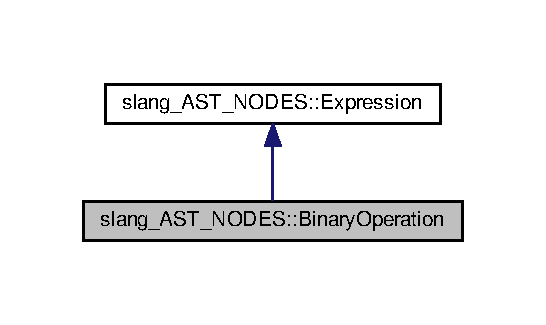
\includegraphics[width=262pt]{classslang__AST__NODES_1_1BinaryOperation__inherit__graph}
\end{center}
\end{figure}


Collaboration diagram for slang\+\_\+\+A\+S\+T\+\_\+\+N\+O\+D\+ES\+:\+:Binary\+Operation\+:
\nopagebreak
\begin{figure}[H]
\begin{center}
\leavevmode
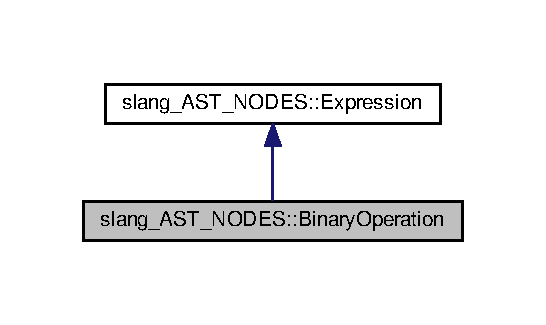
\includegraphics[width=262pt]{classslang__AST__NODES_1_1BinaryOperation__coll__graph}
\end{center}
\end{figure}
\subsection*{Public Types}
\begin{DoxyCompactItemize}
\item 
enum {\bfseries Type} \{ \\*
{\bfseries A\+D\+D\+I\+T\+I\+ON}, 
{\bfseries S\+U\+B\+T\+R\+A\+C\+T\+I\+ON}, 
{\bfseries M\+U\+L\+T\+I\+P\+L\+I\+C\+A\+T\+I\+ON}, 
{\bfseries D\+I\+V\+I\+S\+I\+ON}, 
\\*
{\bfseries M\+O\+D\+U\+LO}, 
{\bfseries P\+OW}, 
{\bfseries A\+S\+S\+I\+GN}, 
{\bfseries E\+Q\+U\+AL}, 
\\*
{\bfseries N\+O\+N\+\_\+\+E\+Q\+U\+AL}, 
{\bfseries G\+R\+E\+AT}, 
{\bfseries G\+R\+E\+A\+T\+\_\+\+E\+Q\+U\+AL}, 
{\bfseries L\+E\+A\+ST}, 
\\*
{\bfseries L\+E\+A\+S\+T\+\_\+\+E\+Q\+U\+AL}, 
{\bfseries A\+ND}, 
{\bfseries OR}
 \}\hypertarget{classslang__AST__NODES_1_1BinaryOperation_ace9b829d1a97c814f923a04027be5bc5}{}\label{classslang__AST__NODES_1_1BinaryOperation_ace9b829d1a97c814f923a04027be5bc5}

\end{DoxyCompactItemize}
\subsection*{Public Member Functions}
\begin{DoxyCompactItemize}
\item 
{\bfseries Binary\+Operation} (Type type\+\_\+, \hyperlink{classslang__AST__NODES_1_1Expression}{Expression} $\ast$first\+Operand\+\_\+, \hyperlink{classslang__AST__NODES_1_1Expression}{Expression} $\ast$second\+Operand\+\_\+)\hypertarget{classslang__AST__NODES_1_1BinaryOperation_a0f81ad9d8548cf8fe9036a1ac2cd946a}{}\label{classslang__AST__NODES_1_1BinaryOperation_a0f81ad9d8548cf8fe9036a1ac2cd946a}

\item 
void {\bfseries print} (F\+I\+LE $\ast$stream) override\hypertarget{classslang__AST__NODES_1_1BinaryOperation_a73846657effdef8eaf520da3e25f61a2}{}\label{classslang__AST__NODES_1_1BinaryOperation_a73846657effdef8eaf520da3e25f61a2}

\end{DoxyCompactItemize}


The documentation for this class was generated from the following file\+:\begin{DoxyCompactItemize}
\item 
src/compiler/parser\+And\+Lexer/ast\+Classes.\+hpp\end{DoxyCompactItemize}

\hypertarget{classslang__AST__NODES_1_1Expression}{}\section{slang\+\_\+\+A\+S\+T\+\_\+\+N\+O\+D\+ES\+:\+:Expression Class Reference}
\label{classslang__AST__NODES_1_1Expression}\index{slang\+\_\+\+A\+S\+T\+\_\+\+N\+O\+D\+E\+S\+::\+Expression@{slang\+\_\+\+A\+S\+T\+\_\+\+N\+O\+D\+E\+S\+::\+Expression}}


Inheritance diagram for slang\+\_\+\+A\+S\+T\+\_\+\+N\+O\+D\+ES\+:\+:Expression\+:
\nopagebreak
\begin{figure}[H]
\begin{center}
\leavevmode
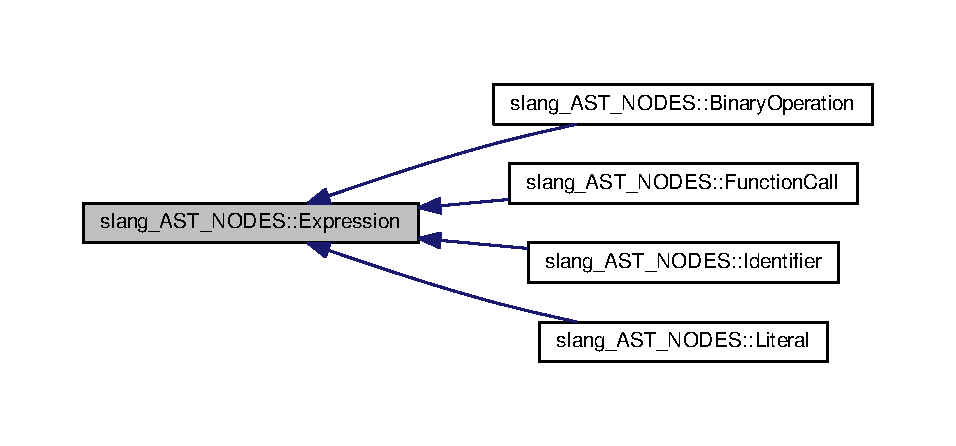
\includegraphics[width=350pt]{classslang__AST__NODES_1_1Expression__inherit__graph}
\end{center}
\end{figure}
\subsection*{Public Member Functions}
\begin{DoxyCompactItemize}
\item 
{\bfseries Expression} (const \hyperlink{classslang__AST__NODES_1_1Expression}{Expression} \&)=delete\hypertarget{classslang__AST__NODES_1_1Expression_a972d3fc6060baa19e37584a3ae5c5014}{}\label{classslang__AST__NODES_1_1Expression_a972d3fc6060baa19e37584a3ae5c5014}

\item 
{\bfseries Expression} (\hyperlink{classslang__AST__NODES_1_1Expression}{Expression} \&\&)=delete\hypertarget{classslang__AST__NODES_1_1Expression_afe4f99a0bf933a442d9a50eb0473345d}{}\label{classslang__AST__NODES_1_1Expression_afe4f99a0bf933a442d9a50eb0473345d}

\item 
void {\bfseries operator=} (const \hyperlink{classslang__AST__NODES_1_1Expression}{Expression} \&)=delete\hypertarget{classslang__AST__NODES_1_1Expression_ac8cbdc46f4947ff17daf3e50ae15780d}{}\label{classslang__AST__NODES_1_1Expression_ac8cbdc46f4947ff17daf3e50ae15780d}

\item 
void {\bfseries operator=} (\hyperlink{classslang__AST__NODES_1_1Expression}{Expression} \&\&)=delete\hypertarget{classslang__AST__NODES_1_1Expression_a4a8542aab7b4f00673dc922e7cd17bcc}{}\label{classslang__AST__NODES_1_1Expression_a4a8542aab7b4f00673dc922e7cd17bcc}

\item 
virtual void {\bfseries print} (F\+I\+LE $\ast$stream)=0\hypertarget{classslang__AST__NODES_1_1Expression_a1e7354a0f66c6096a787fbed0cc98537}{}\label{classslang__AST__NODES_1_1Expression_a1e7354a0f66c6096a787fbed0cc98537}

\end{DoxyCompactItemize}


The documentation for this class was generated from the following file\+:\begin{DoxyCompactItemize}
\item 
src/compiler/parser\+And\+Lexer/ast\+Classes.\+hpp\end{DoxyCompactItemize}

\hypertarget{classslang__AST__NODES_1_1ForLoop}{}\section{slang\+\_\+\+A\+S\+T\+\_\+\+N\+O\+D\+ES\+:\+:For\+Loop Class Reference}
\label{classslang__AST__NODES_1_1ForLoop}\index{slang\+\_\+\+A\+S\+T\+\_\+\+N\+O\+D\+E\+S\+::\+For\+Loop@{slang\+\_\+\+A\+S\+T\+\_\+\+N\+O\+D\+E\+S\+::\+For\+Loop}}


Inheritance diagram for slang\+\_\+\+A\+S\+T\+\_\+\+N\+O\+D\+ES\+:\+:For\+Loop\+:
\nopagebreak
\begin{figure}[H]
\begin{center}
\leavevmode
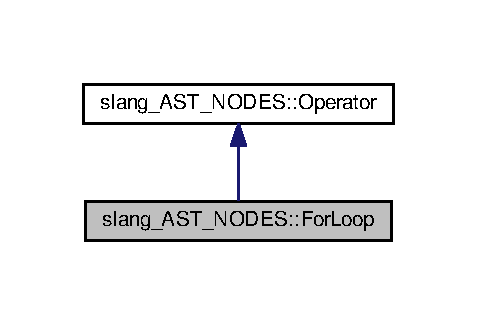
\includegraphics[width=229pt]{classslang__AST__NODES_1_1ForLoop__inherit__graph}
\end{center}
\end{figure}


Collaboration diagram for slang\+\_\+\+A\+S\+T\+\_\+\+N\+O\+D\+ES\+:\+:For\+Loop\+:
\nopagebreak
\begin{figure}[H]
\begin{center}
\leavevmode
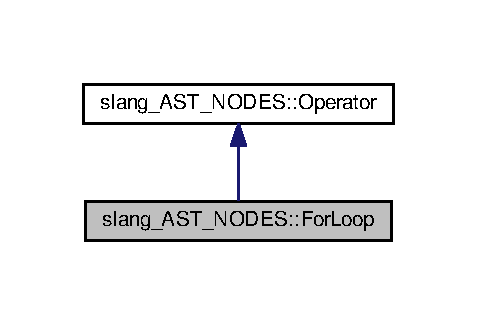
\includegraphics[width=229pt]{classslang__AST__NODES_1_1ForLoop__coll__graph}
\end{center}
\end{figure}
\subsection*{Public Member Functions}
\begin{DoxyCompactItemize}
\item 
{\bfseries For\+Loop} (\hyperlink{classslang__AST__NODES_1_1Expression}{Expression} $\ast$first\+Expr\+\_\+, \hyperlink{classslang__AST__NODES_1_1Expression}{Expression} $\ast$second\+Expr\+\_\+, \hyperlink{classslang__AST__NODES_1_1Expression}{Expression} $\ast$third\+Expr\+\_\+, \hyperlink{classslang__AST__NODES_1_1Operator}{Operator} $\ast$body\+\_\+)\hypertarget{classslang__AST__NODES_1_1ForLoop_ad14ac995f22bc6ddddf40374a4225202}{}\label{classslang__AST__NODES_1_1ForLoop_ad14ac995f22bc6ddddf40374a4225202}

\item 
void {\bfseries print} (F\+I\+LE $\ast$stream, int indent\+Level) override\hypertarget{classslang__AST__NODES_1_1ForLoop_a92ccb559c47928fd9eb290b2e8dd9972}{}\label{classslang__AST__NODES_1_1ForLoop_a92ccb559c47928fd9eb290b2e8dd9972}

\end{DoxyCompactItemize}


The documentation for this class was generated from the following file\+:\begin{DoxyCompactItemize}
\item 
src/compiler/parser\+And\+Lexer/ast\+Classes.\+hpp\end{DoxyCompactItemize}

\hypertarget{classslang__AST__NODES_1_1Function}{}\section{slang\+\_\+\+A\+S\+T\+\_\+\+N\+O\+D\+ES\+:\+:Function Class Reference}
\label{classslang__AST__NODES_1_1Function}\index{slang\+\_\+\+A\+S\+T\+\_\+\+N\+O\+D\+E\+S\+::\+Function@{slang\+\_\+\+A\+S\+T\+\_\+\+N\+O\+D\+E\+S\+::\+Function}}
\subsection*{Public Member Functions}
\begin{DoxyCompactItemize}
\item 
{\bfseries Function} (std\+::string name\+\_\+, std\+::vector$<$ \hyperlink{classslang__AST__NODES_1_1Identifier}{Identifier} $\ast$ $>$ parameters\+Name\+\_\+, \hyperlink{classslang__AST__NODES_1_1Operator}{Operator} $\ast$body\+\_\+)\hypertarget{classslang__AST__NODES_1_1Function_a1b5f28e8b549cc3604104b37aac028b5}{}\label{classslang__AST__NODES_1_1Function_a1b5f28e8b549cc3604104b37aac028b5}

\end{DoxyCompactItemize}


The documentation for this class was generated from the following file\+:\begin{DoxyCompactItemize}
\item 
src/compiler/parser\+And\+Lexer/ast\+Classes.\+hpp\end{DoxyCompactItemize}

\hypertarget{classslang__AST__NODES_1_1FunctionCall}{}\section{slang\+\_\+\+A\+S\+T\+\_\+\+N\+O\+D\+ES\+:\+:Function\+Call Class Reference}
\label{classslang__AST__NODES_1_1FunctionCall}\index{slang\+\_\+\+A\+S\+T\+\_\+\+N\+O\+D\+E\+S\+::\+Function\+Call@{slang\+\_\+\+A\+S\+T\+\_\+\+N\+O\+D\+E\+S\+::\+Function\+Call}}


Inheritance diagram for slang\+\_\+\+A\+S\+T\+\_\+\+N\+O\+D\+ES\+:\+:Function\+Call\+:
\nopagebreak
\begin{figure}[H]
\begin{center}
\leavevmode
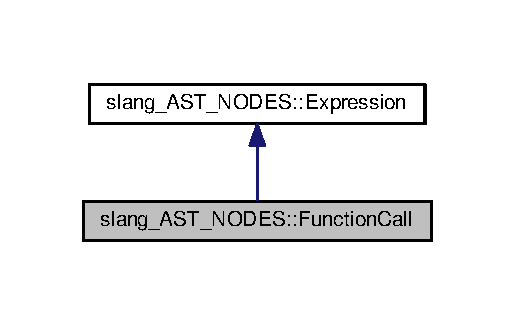
\includegraphics[width=247pt]{classslang__AST__NODES_1_1FunctionCall__inherit__graph}
\end{center}
\end{figure}


Collaboration diagram for slang\+\_\+\+A\+S\+T\+\_\+\+N\+O\+D\+ES\+:\+:Function\+Call\+:
\nopagebreak
\begin{figure}[H]
\begin{center}
\leavevmode
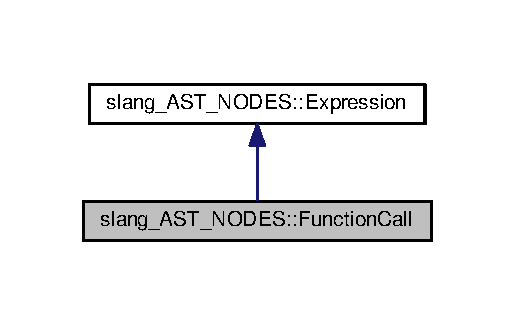
\includegraphics[width=247pt]{classslang__AST__NODES_1_1FunctionCall__coll__graph}
\end{center}
\end{figure}
\subsection*{Public Member Functions}
\begin{DoxyCompactItemize}
\item 
{\bfseries Function\+Call} (std\+::string name\+\_\+, std\+::vector$<$ \hyperlink{classslang__AST__NODES_1_1Expression}{Expression} $\ast$ $>$ arguments\+\_\+)\hypertarget{classslang__AST__NODES_1_1FunctionCall_a02b913fb8644a160f3122dd6fef284b6}{}\label{classslang__AST__NODES_1_1FunctionCall_a02b913fb8644a160f3122dd6fef284b6}

\item 
void {\bfseries print} (F\+I\+LE $\ast$stream) override\hypertarget{classslang__AST__NODES_1_1FunctionCall_a23baa8b7ddd506c72072df66af4ccbdd}{}\label{classslang__AST__NODES_1_1FunctionCall_a23baa8b7ddd506c72072df66af4ccbdd}

\end{DoxyCompactItemize}


The documentation for this class was generated from the following file\+:\begin{DoxyCompactItemize}
\item 
src/compiler/parser\+And\+Lexer/ast\+Classes.\+hpp\end{DoxyCompactItemize}

\hypertarget{classslang__AST__NODES_1_1Identifier}{}\section{slang\+\_\+\+A\+S\+T\+\_\+\+N\+O\+D\+ES\+:\+:Identifier Class Reference}
\label{classslang__AST__NODES_1_1Identifier}\index{slang\+\_\+\+A\+S\+T\+\_\+\+N\+O\+D\+E\+S\+::\+Identifier@{slang\+\_\+\+A\+S\+T\+\_\+\+N\+O\+D\+E\+S\+::\+Identifier}}


Inheritance diagram for slang\+\_\+\+A\+S\+T\+\_\+\+N\+O\+D\+ES\+:\+:Identifier\+:
\nopagebreak
\begin{figure}[H]
\begin{center}
\leavevmode
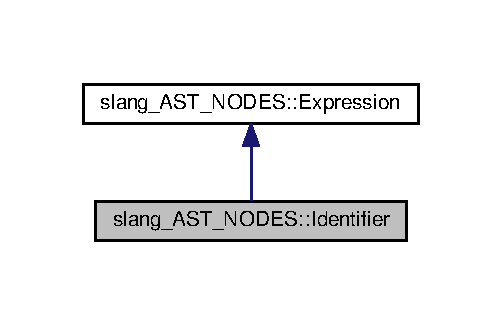
\includegraphics[width=241pt]{classslang__AST__NODES_1_1Identifier__inherit__graph}
\end{center}
\end{figure}


Collaboration diagram for slang\+\_\+\+A\+S\+T\+\_\+\+N\+O\+D\+ES\+:\+:Identifier\+:
\nopagebreak
\begin{figure}[H]
\begin{center}
\leavevmode
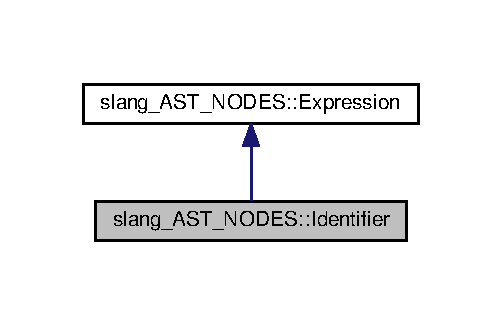
\includegraphics[width=241pt]{classslang__AST__NODES_1_1Identifier__coll__graph}
\end{center}
\end{figure}
\subsection*{Public Member Functions}
\begin{DoxyCompactItemize}
\item 
{\bfseries Identifier} (const std\+::string value\+\_\+)\hypertarget{classslang__AST__NODES_1_1Identifier_a0d0049f7138996421c62abdd486cc0bc}{}\label{classslang__AST__NODES_1_1Identifier_a0d0049f7138996421c62abdd486cc0bc}

\item 
void {\bfseries print} (F\+I\+LE $\ast$stream) override\hypertarget{classslang__AST__NODES_1_1Identifier_ad40c1bcac8d970fa97337fac84e70873}{}\label{classslang__AST__NODES_1_1Identifier_ad40c1bcac8d970fa97337fac84e70873}

\end{DoxyCompactItemize}


The documentation for this class was generated from the following file\+:\begin{DoxyCompactItemize}
\item 
src/compiler/parser\+And\+Lexer/ast\+Classes.\+hpp\end{DoxyCompactItemize}

\hypertarget{classslang__AST__NODES_1_1Literal}{}\section{slang\+\_\+\+A\+S\+T\+\_\+\+N\+O\+D\+ES\+:\+:Literal Class Reference}
\label{classslang__AST__NODES_1_1Literal}\index{slang\+\_\+\+A\+S\+T\+\_\+\+N\+O\+D\+E\+S\+::\+Literal@{slang\+\_\+\+A\+S\+T\+\_\+\+N\+O\+D\+E\+S\+::\+Literal}}


Inheritance diagram for slang\+\_\+\+A\+S\+T\+\_\+\+N\+O\+D\+ES\+:\+:Literal\+:
\nopagebreak
\begin{figure}[H]
\begin{center}
\leavevmode
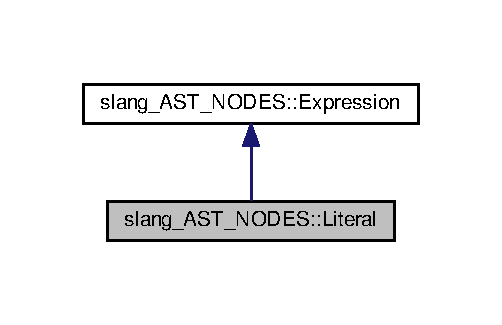
\includegraphics[width=241pt]{classslang__AST__NODES_1_1Literal__inherit__graph}
\end{center}
\end{figure}


Collaboration diagram for slang\+\_\+\+A\+S\+T\+\_\+\+N\+O\+D\+ES\+:\+:Literal\+:
\nopagebreak
\begin{figure}[H]
\begin{center}
\leavevmode
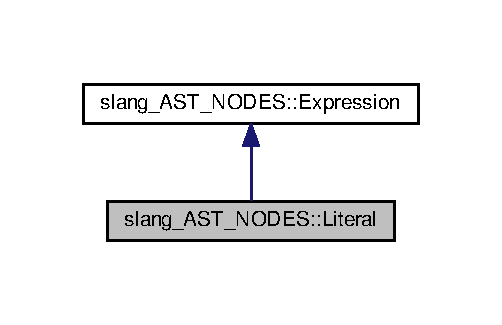
\includegraphics[width=241pt]{classslang__AST__NODES_1_1Literal__coll__graph}
\end{center}
\end{figure}
\subsection*{Public Member Functions}
\begin{DoxyCompactItemize}
\item 
{\bfseries Literal} (const int val)\hypertarget{classslang__AST__NODES_1_1Literal_ad798bc229c978a146e476e373ab11b3d}{}\label{classslang__AST__NODES_1_1Literal_ad798bc229c978a146e476e373ab11b3d}

\item 
{\bfseries Literal} (const double val)\hypertarget{classslang__AST__NODES_1_1Literal_a427c1a12545ba81884e4a28829c0a757}{}\label{classslang__AST__NODES_1_1Literal_a427c1a12545ba81884e4a28829c0a757}

\item 
{\bfseries Literal} (const bool val)\hypertarget{classslang__AST__NODES_1_1Literal_a552dcdbe04750ac46bdac2ffb984cef2}{}\label{classslang__AST__NODES_1_1Literal_a552dcdbe04750ac46bdac2ffb984cef2}

\item 
{\bfseries Literal} (const std\+::string val)\hypertarget{classslang__AST__NODES_1_1Literal_a3abd91746cd21ef8ddf6e0309655085e}{}\label{classslang__AST__NODES_1_1Literal_a3abd91746cd21ef8ddf6e0309655085e}

\item 
{\bfseries Literal} (const char val)\hypertarget{classslang__AST__NODES_1_1Literal_aa7c179a9b9697ff1bf5b2f3bc4805aaa}{}\label{classslang__AST__NODES_1_1Literal_aa7c179a9b9697ff1bf5b2f3bc4805aaa}

\item 
void {\bfseries print} (F\+I\+LE $\ast$stream) override\hypertarget{classslang__AST__NODES_1_1Literal_ac50bf74dc205581b39c5ea297ba6a6c4}{}\label{classslang__AST__NODES_1_1Literal_ac50bf74dc205581b39c5ea297ba6a6c4}

\end{DoxyCompactItemize}


The documentation for this class was generated from the following file\+:\begin{DoxyCompactItemize}
\item 
src/compiler/parser\+And\+Lexer/ast\+Classes.\+hpp\end{DoxyCompactItemize}

\hypertarget{classslang__AST__NODES_1_1Operator}{}\section{slang\+\_\+\+A\+S\+T\+\_\+\+N\+O\+D\+ES\+:\+:Operator Class Reference}
\label{classslang__AST__NODES_1_1Operator}\index{slang\+\_\+\+A\+S\+T\+\_\+\+N\+O\+D\+E\+S\+::\+Operator@{slang\+\_\+\+A\+S\+T\+\_\+\+N\+O\+D\+E\+S\+::\+Operator}}


Inheritance diagram for slang\+\_\+\+A\+S\+T\+\_\+\+N\+O\+D\+ES\+:\+:Operator\+:
\nopagebreak
\begin{figure}[H]
\begin{center}
\leavevmode
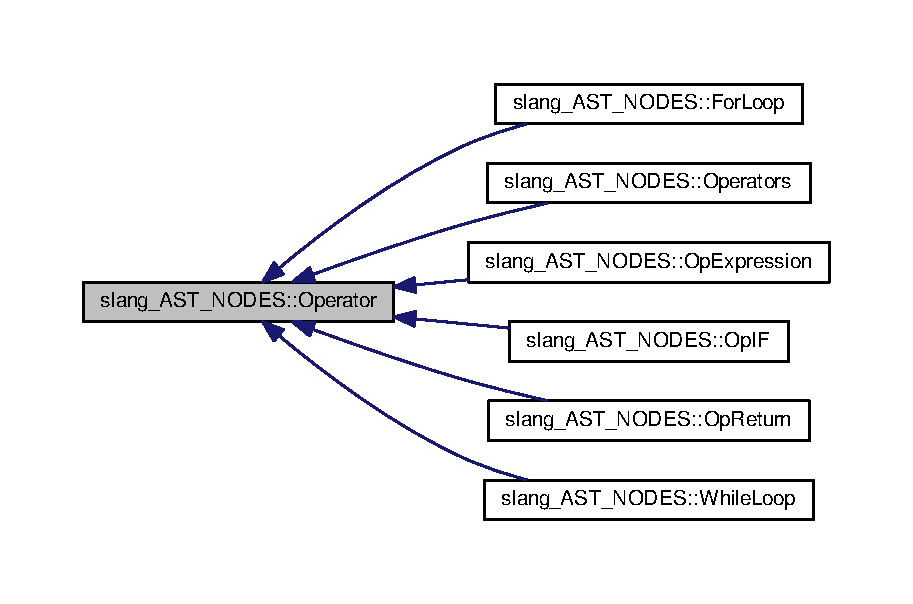
\includegraphics[width=350pt]{classslang__AST__NODES_1_1Operator__inherit__graph}
\end{center}
\end{figure}
\subsection*{Public Member Functions}
\begin{DoxyCompactItemize}
\item 
{\bfseries Operator} (const \hyperlink{classslang__AST__NODES_1_1Operator}{Operator} \&)=delete\hypertarget{classslang__AST__NODES_1_1Operator_a2133487159af1697624113aee8cdf0fe}{}\label{classslang__AST__NODES_1_1Operator_a2133487159af1697624113aee8cdf0fe}

\item 
{\bfseries Operator} (\hyperlink{classslang__AST__NODES_1_1Operator}{Operator} \&\&)=delete\hypertarget{classslang__AST__NODES_1_1Operator_a3e5978ea07f080b1f02d974b490fda88}{}\label{classslang__AST__NODES_1_1Operator_a3e5978ea07f080b1f02d974b490fda88}

\item 
void {\bfseries operator=} (const \hyperlink{classslang__AST__NODES_1_1Operator}{Operator} \&)=delete\hypertarget{classslang__AST__NODES_1_1Operator_ac4bdfbee38f554f4ddb2b0463417cd18}{}\label{classslang__AST__NODES_1_1Operator_ac4bdfbee38f554f4ddb2b0463417cd18}

\item 
void {\bfseries operator=} (\hyperlink{classslang__AST__NODES_1_1Operator}{Operator} \&\&)=delete\hypertarget{classslang__AST__NODES_1_1Operator_ad9cc76b721856b7e731d4a1dfb5a986b}{}\label{classslang__AST__NODES_1_1Operator_ad9cc76b721856b7e731d4a1dfb5a986b}

\item 
virtual void {\bfseries print} (F\+I\+LE $\ast$stream, int indent\+Level)=0\hypertarget{classslang__AST__NODES_1_1Operator_ae09e8d2fb6dfe2eb76acf11e5b60bfe0}{}\label{classslang__AST__NODES_1_1Operator_ae09e8d2fb6dfe2eb76acf11e5b60bfe0}

\item 
void {\bfseries print\+Indent} (int level, F\+I\+LE $\ast$stream)\hypertarget{classslang__AST__NODES_1_1Operator_a55dea6860e708b5bfdfc4f93af1f6370}{}\label{classslang__AST__NODES_1_1Operator_a55dea6860e708b5bfdfc4f93af1f6370}

\end{DoxyCompactItemize}


The documentation for this class was generated from the following file\+:\begin{DoxyCompactItemize}
\item 
src/compiler/parser\+And\+Lexer/ast\+Classes.\+hpp\end{DoxyCompactItemize}

\hypertarget{classslang__AST__NODES_1_1Operators}{}\section{slang\+\_\+\+A\+S\+T\+\_\+\+N\+O\+D\+ES\+:\+:Operators Class Reference}
\label{classslang__AST__NODES_1_1Operators}\index{slang\+\_\+\+A\+S\+T\+\_\+\+N\+O\+D\+E\+S\+::\+Operators@{slang\+\_\+\+A\+S\+T\+\_\+\+N\+O\+D\+E\+S\+::\+Operators}}


Inheritance diagram for slang\+\_\+\+A\+S\+T\+\_\+\+N\+O\+D\+ES\+:\+:Operators\+:
\nopagebreak
\begin{figure}[H]
\begin{center}
\leavevmode
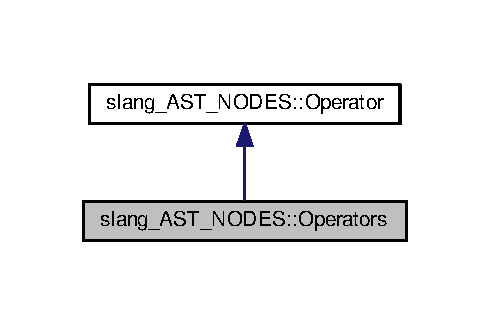
\includegraphics[width=235pt]{classslang__AST__NODES_1_1Operators__inherit__graph}
\end{center}
\end{figure}


Collaboration diagram for slang\+\_\+\+A\+S\+T\+\_\+\+N\+O\+D\+ES\+:\+:Operators\+:
\nopagebreak
\begin{figure}[H]
\begin{center}
\leavevmode
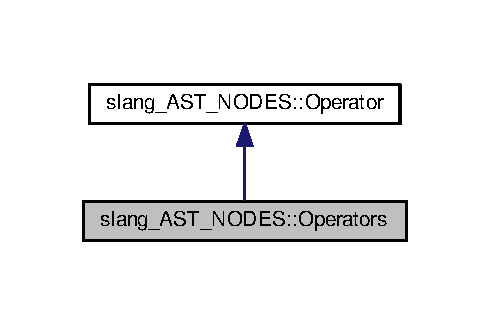
\includegraphics[width=235pt]{classslang__AST__NODES_1_1Operators__coll__graph}
\end{center}
\end{figure}
\subsection*{Public Member Functions}
\begin{DoxyCompactItemize}
\item 
void {\bfseries push\+\_\+back} (\hyperlink{classslang__AST__NODES_1_1Operator}{Operator} $\ast$op)\hypertarget{classslang__AST__NODES_1_1Operators_a5243e6b675f569df2ed4a2afbb073814}{}\label{classslang__AST__NODES_1_1Operators_a5243e6b675f569df2ed4a2afbb073814}

\item 
void {\bfseries print} (F\+I\+LE $\ast$stream, int indent\+Level) override\hypertarget{classslang__AST__NODES_1_1Operators_a981d00f1e44e2f840648993dc99ec781}{}\label{classslang__AST__NODES_1_1Operators_a981d00f1e44e2f840648993dc99ec781}

\end{DoxyCompactItemize}


The documentation for this class was generated from the following file\+:\begin{DoxyCompactItemize}
\item 
src/compiler/parser\+And\+Lexer/ast\+Classes.\+hpp\end{DoxyCompactItemize}

\hypertarget{classslang__AST__NODES_1_1OpExpression}{}\section{slang\+\_\+\+A\+S\+T\+\_\+\+N\+O\+D\+ES\+:\+:Op\+Expression Class Reference}
\label{classslang__AST__NODES_1_1OpExpression}\index{slang\+\_\+\+A\+S\+T\+\_\+\+N\+O\+D\+E\+S\+::\+Op\+Expression@{slang\+\_\+\+A\+S\+T\+\_\+\+N\+O\+D\+E\+S\+::\+Op\+Expression}}


Inheritance diagram for slang\+\_\+\+A\+S\+T\+\_\+\+N\+O\+D\+ES\+:\+:Op\+Expression\+:
\nopagebreak
\begin{figure}[H]
\begin{center}
\leavevmode
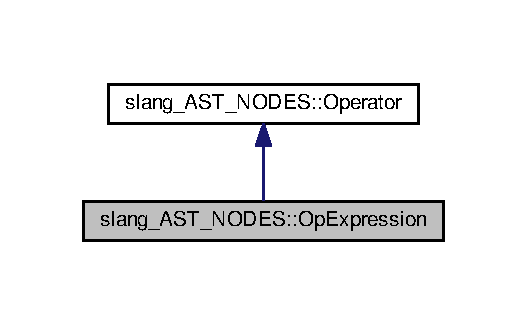
\includegraphics[width=253pt]{classslang__AST__NODES_1_1OpExpression__inherit__graph}
\end{center}
\end{figure}


Collaboration diagram for slang\+\_\+\+A\+S\+T\+\_\+\+N\+O\+D\+ES\+:\+:Op\+Expression\+:
\nopagebreak
\begin{figure}[H]
\begin{center}
\leavevmode
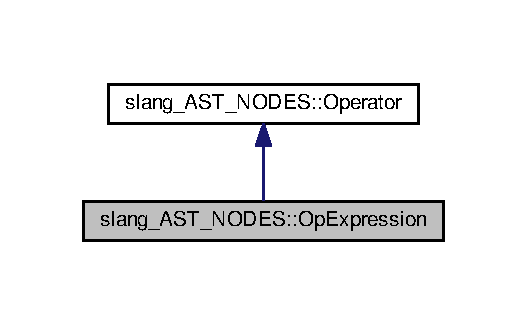
\includegraphics[width=253pt]{classslang__AST__NODES_1_1OpExpression__coll__graph}
\end{center}
\end{figure}
\subsection*{Public Member Functions}
\begin{DoxyCompactItemize}
\item 
{\bfseries Op\+Expression} (\hyperlink{classslang__AST__NODES_1_1Expression}{Expression} $\ast$e)\hypertarget{classslang__AST__NODES_1_1OpExpression_a870357f321a081a5052a3c0f312a77bf}{}\label{classslang__AST__NODES_1_1OpExpression_a870357f321a081a5052a3c0f312a77bf}

\item 
void {\bfseries print} (F\+I\+LE $\ast$stream, int indent\+Level) override\hypertarget{classslang__AST__NODES_1_1OpExpression_a6e39980dad216f83c4cc52609d80bd39}{}\label{classslang__AST__NODES_1_1OpExpression_a6e39980dad216f83c4cc52609d80bd39}

\end{DoxyCompactItemize}


The documentation for this class was generated from the following file\+:\begin{DoxyCompactItemize}
\item 
src/compiler/parser\+And\+Lexer/ast\+Classes.\+hpp\end{DoxyCompactItemize}

\hypertarget{classslang__AST__NODES_1_1OpIF}{}\section{slang\+\_\+\+A\+S\+T\+\_\+\+N\+O\+D\+ES\+:\+:Op\+IF Class Reference}
\label{classslang__AST__NODES_1_1OpIF}\index{slang\+\_\+\+A\+S\+T\+\_\+\+N\+O\+D\+E\+S\+::\+Op\+IF@{slang\+\_\+\+A\+S\+T\+\_\+\+N\+O\+D\+E\+S\+::\+Op\+IF}}


Inheritance diagram for slang\+\_\+\+A\+S\+T\+\_\+\+N\+O\+D\+ES\+:\+:Op\+IF\+:
\nopagebreak
\begin{figure}[H]
\begin{center}
\leavevmode
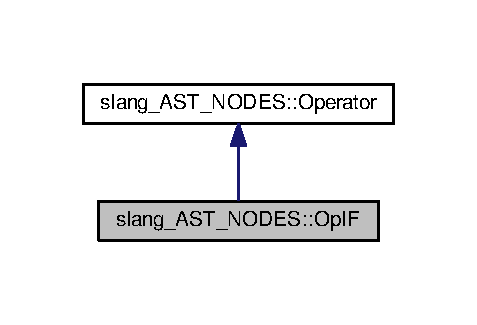
\includegraphics[width=229pt]{classslang__AST__NODES_1_1OpIF__inherit__graph}
\end{center}
\end{figure}


Collaboration diagram for slang\+\_\+\+A\+S\+T\+\_\+\+N\+O\+D\+ES\+:\+:Op\+IF\+:
\nopagebreak
\begin{figure}[H]
\begin{center}
\leavevmode
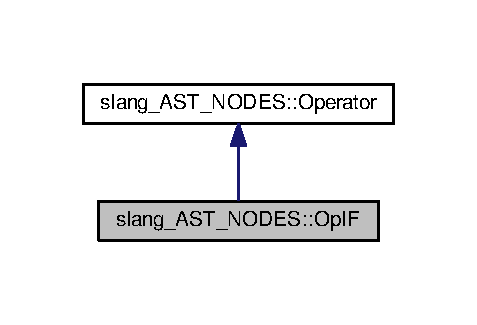
\includegraphics[width=229pt]{classslang__AST__NODES_1_1OpIF__coll__graph}
\end{center}
\end{figure}
\subsection*{Public Member Functions}
\begin{DoxyCompactItemize}
\item 
{\bfseries Op\+IF} (\hyperlink{classslang__AST__NODES_1_1Expression}{Expression} $\ast$cond, \hyperlink{classslang__AST__NODES_1_1Operator}{Operator} $\ast$if\+Op\+\_\+, \hyperlink{classslang__AST__NODES_1_1Operator}{Operator} $\ast$else\+Op\+\_\+)\hypertarget{classslang__AST__NODES_1_1OpIF_a77a112bc398c4594cbdbf7e5c8a9929e}{}\label{classslang__AST__NODES_1_1OpIF_a77a112bc398c4594cbdbf7e5c8a9929e}

\item 
{\bfseries Op\+IF} (\hyperlink{classslang__AST__NODES_1_1Expression}{Expression} $\ast$cond, \hyperlink{classslang__AST__NODES_1_1Operator}{Operator} $\ast$if\+Op\+\_\+)\hypertarget{classslang__AST__NODES_1_1OpIF_ac45b7c8e8412ecabc7d4cba9c45fa71f}{}\label{classslang__AST__NODES_1_1OpIF_ac45b7c8e8412ecabc7d4cba9c45fa71f}

\item 
void {\bfseries print} (F\+I\+LE $\ast$stream, int indent\+Level)\hypertarget{classslang__AST__NODES_1_1OpIF_a6cc095933d18ded2278145c760629bb5}{}\label{classslang__AST__NODES_1_1OpIF_a6cc095933d18ded2278145c760629bb5}

\end{DoxyCompactItemize}


The documentation for this class was generated from the following file\+:\begin{DoxyCompactItemize}
\item 
src/compiler/parser\+And\+Lexer/ast\+Classes.\+hpp\end{DoxyCompactItemize}

\hypertarget{classslang__AST__NODES_1_1OpReturn}{}\section{slang\+\_\+\+A\+S\+T\+\_\+\+N\+O\+D\+ES\+:\+:Op\+Return Class Reference}
\label{classslang__AST__NODES_1_1OpReturn}\index{slang\+\_\+\+A\+S\+T\+\_\+\+N\+O\+D\+E\+S\+::\+Op\+Return@{slang\+\_\+\+A\+S\+T\+\_\+\+N\+O\+D\+E\+S\+::\+Op\+Return}}


Inheritance diagram for slang\+\_\+\+A\+S\+T\+\_\+\+N\+O\+D\+ES\+:\+:Op\+Return\+:
\nopagebreak
\begin{figure}[H]
\begin{center}
\leavevmode
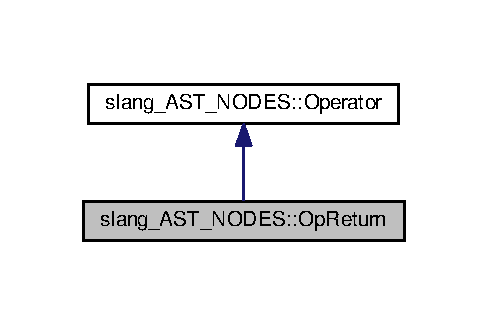
\includegraphics[width=234pt]{classslang__AST__NODES_1_1OpReturn__inherit__graph}
\end{center}
\end{figure}


Collaboration diagram for slang\+\_\+\+A\+S\+T\+\_\+\+N\+O\+D\+ES\+:\+:Op\+Return\+:
\nopagebreak
\begin{figure}[H]
\begin{center}
\leavevmode
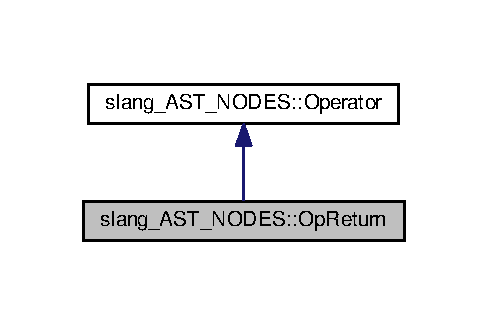
\includegraphics[width=234pt]{classslang__AST__NODES_1_1OpReturn__coll__graph}
\end{center}
\end{figure}
\subsection*{Public Member Functions}
\begin{DoxyCompactItemize}
\item 
{\bfseries Op\+Return} (\hyperlink{classslang__AST__NODES_1_1Expression}{Expression} $\ast$e)\hypertarget{classslang__AST__NODES_1_1OpReturn_a2338b3b04ae0ee23736ece5d04d8d121}{}\label{classslang__AST__NODES_1_1OpReturn_a2338b3b04ae0ee23736ece5d04d8d121}

\item 
void {\bfseries print} (F\+I\+LE $\ast$stream, int indent\+Level) override\hypertarget{classslang__AST__NODES_1_1OpReturn_aa76bf80d86ada5e7cd269d2dc34a9ad4}{}\label{classslang__AST__NODES_1_1OpReturn_aa76bf80d86ada5e7cd269d2dc34a9ad4}

\end{DoxyCompactItemize}


The documentation for this class was generated from the following file\+:\begin{DoxyCompactItemize}
\item 
src/compiler/parser\+And\+Lexer/ast\+Classes.\+hpp\end{DoxyCompactItemize}

\hypertarget{classslang__AST__NODES_1_1WhileLoop}{}\section{slang\+\_\+\+A\+S\+T\+\_\+\+N\+O\+D\+ES\+:\+:While\+Loop Class Reference}
\label{classslang__AST__NODES_1_1WhileLoop}\index{slang\+\_\+\+A\+S\+T\+\_\+\+N\+O\+D\+E\+S\+::\+While\+Loop@{slang\+\_\+\+A\+S\+T\+\_\+\+N\+O\+D\+E\+S\+::\+While\+Loop}}


Inheritance diagram for slang\+\_\+\+A\+S\+T\+\_\+\+N\+O\+D\+ES\+:\+:While\+Loop\+:
\nopagebreak
\begin{figure}[H]
\begin{center}
\leavevmode
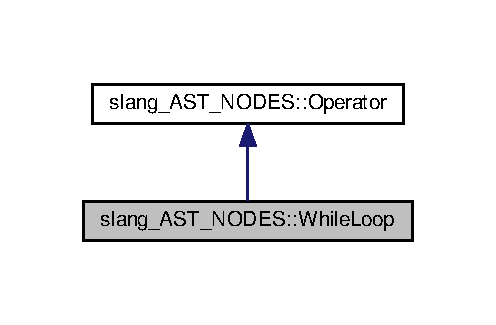
\includegraphics[width=238pt]{classslang__AST__NODES_1_1WhileLoop__inherit__graph}
\end{center}
\end{figure}


Collaboration diagram for slang\+\_\+\+A\+S\+T\+\_\+\+N\+O\+D\+ES\+:\+:While\+Loop\+:
\nopagebreak
\begin{figure}[H]
\begin{center}
\leavevmode
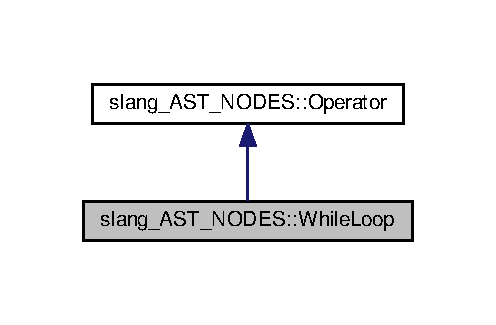
\includegraphics[width=238pt]{classslang__AST__NODES_1_1WhileLoop__coll__graph}
\end{center}
\end{figure}
\subsection*{Public Member Functions}
\begin{DoxyCompactItemize}
\item 
{\bfseries While\+Loop} (\hyperlink{classslang__AST__NODES_1_1Expression}{Expression} $\ast$condition\+\_\+, \hyperlink{classslang__AST__NODES_1_1Operator}{Operator} $\ast$body\+\_\+)\hypertarget{classslang__AST__NODES_1_1WhileLoop_ac15e8e4d71c95a9a13cfd40d3f2490c0}{}\label{classslang__AST__NODES_1_1WhileLoop_ac15e8e4d71c95a9a13cfd40d3f2490c0}

\item 
void {\bfseries print} (F\+I\+LE $\ast$stream, int indent\+Level) override\hypertarget{classslang__AST__NODES_1_1WhileLoop_ace71f78e29b6b80620d9d82b676632e8}{}\label{classslang__AST__NODES_1_1WhileLoop_ace71f78e29b6b80620d9d82b676632e8}

\end{DoxyCompactItemize}


The documentation for this class was generated from the following file\+:\begin{DoxyCompactItemize}
\item 
src/compiler/parser\+And\+Lexer/ast\+Classes.\+hpp\end{DoxyCompactItemize}

%--- End generated contents ---

% Index
\backmatter
\newpage
\phantomsection
\clearemptydoublepage
\addcontentsline{toc}{chapter}{Index}
\printindex

\end{document}
